\subsection{PID Controller}
    \subsubsection{P-Controller}
        \titel{Gain}
            \begin{align*}
                y(t) = u(t)
            \end{align*}
        \begin{itemize}
            \item proportional to error
            \item shifts magnitude, phase unaffected
            \item higher proportional gain moves crossover frequency up
            \item $k_P$ increases:
            \begin{itemize}
                \item closed-loop system of 2nd and higher order become more oscillatory
                \item closed-loop system remains stable
                \item $e_{ss}$ decreases
                \item faster response
                \item increased sensitivity to noise
            \end{itemize}
        \end{itemize}

    \subsubsection{I-Controller (integral)}
        \titel{Integrator}
            \begin{align*}
                y(t) = \int u(t) dt = \int e^{st} dt = \frac{1}{s} \cdot e^{st} = \frac{1}{s} \cdot u(t)
            \end{align*}
            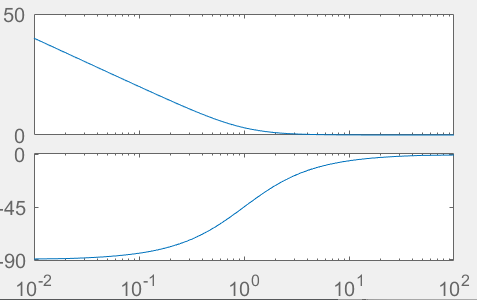
\includegraphics[width = \linewidth]{src/images/PI-controller.png}
        \begin{itemize}
            \item proportional to accumulated error
            \item new zero introduced
            \item number of asymptotes is reduced
            \item steady state error to step input\textbf{exactly zero}
            \item $k_I$ increases:
            \begin{itemize}
                \item more oscillatory response
                \item noise sensitivity does not change
            \end{itemize}
        \end{itemize}

    \subsubsection{D-Controller (derivative)}
        \titel{Differentiator}
            \begin{align*}
                y(t) = \frac{d u(t)}{dt} = \frac{d}{dt} e^{st} = s \cdot e^{st} = s \cdot u(t)
            \end{align*}
            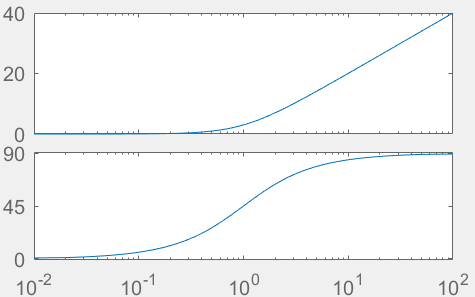
\includegraphics[width = \linewidth]{src/images/PD-controller.png}
        \begin{itemize}
            \item proportional to rate of change of error (reduced overshoot)
            \item pole introduced at $p=0$
            \item zero introduced at $z = -\frac{k_i}{k_p}$
            \item number of asymptotes unchanged
            \item $k_P$ increases:
            \begin{itemize}
                \item $e_{ss}$ unaffected
                \item less oscillatory, but potentially slower
                \item increased sensitivity to noise
            \end{itemize}
        \end{itemize}

    \subsubsection{Building the controller}
        \begin{minipage}{0.49\linewidth}
            \begin{align*}
                C(s) &= k_P + \frac{k_I}{s} + k_D \cdot s\\
                &= \frac{k_P \cdot s + k_I + k_D \cdot s^2}{s}\\
                &= k_P(1 + \frac{1}{T_I \cdot s} + T_D \cdot s)
            \end{align*}
        \end{minipage}
        \begin{minipage}{0.49\linewidth}
            \begin{scriptsize}
                \begin{align*}
                    k_P &= \text{Proportional gain}\\
                    k_I &= \text{Integral gain}\\
                    k_D &= \text{Derivative gain}\\
                    T_I &= \text{Integral time constant gain}\\
                    T_D &= \text{Derivative time constant}
                \end{align*}
            \end{scriptsize}
        \end{minipage}
        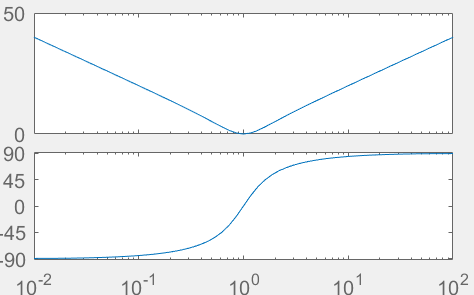
\includegraphics[width = \linewidth]{src/images/PID-controller.png}
        %Von ZF: P-controller, I-controller, D-controller